%
% latex-sample.tex
%
% This LaTeX source file provides a template for a typical research paper.
%

%
% Use the standard article template.
%
\documentclass{article}

% The geometry package allows for easy page formatting.
\usepackage{geometry}
\geometry{letterpaper}

% Load up special logo commands.
\usepackage{doc}
\usepackage{cite}
\usepackage[margin=1cm]{caption}

% Package for formatting URLs.
\usepackage{url}

% Packages and definitions for graphics files.
\usepackage{graphicx}
\usepackage{epstopdf}
\DeclareGraphicsRule{.tif}{png}{.png}{`convert #1 `dirname #1`/`basename #1 .tif`.png}

%
% Set the title, author, and date.
%
\title{Usability of Modern Display Technologies}
\author{Rachel Rivera}
\date{October 16, 2014}

%
% The document proper.
%
\begin{document}

% Add the title section.
\maketitle

% Add an abstract.
\abstract{
This study aims to examine how interaction design concepts specifically map to the usability of modern display technology.
//TODO: write a better abstract
}

% Add various lists on new pages.
\pagebreak
\tableofcontents


% Start the paper on a new page.
\pagebreak

%
% Body text.
%
\section{Introduction}
\label{introduction}

Electronic screens are the devices through which information is transferred between users and the interface. In the same way screens are an imperative component of user interaction with a device, the study of screens is an imperative component of the field of interaction design.

Although electronic displays have been around for nearly a century,\footnote{The cathode ray tube (CRT) was first made commercial in 1922.\cite{Cathode}} they are still transforming and evolving in a multitude of ways. Screens are diversifying in order to tackle the limitations that have presented themselves over the years. Screen devices have been changing in size, shape, flexibility, and resolution in order to improve usability for specific tasks. For example, \textit{focus plus context screens}, which are wall-size low-resolution displays with an embedded high-resolution display region, are currently a proposed solution to working with visual documents too large to fit standard screens.\cite{Baudisch} Another kind of screen that is emerging is the \textit{BiDirectional (BiDi) Screen}, which is a thin, depth-sensing liquid-crystal display (LCD) that allows for 3D interaction using light fields.\cite{Hirsch}

 Though each kind of screen has its merits, this study will focus exclusively on touch sensitive screens. In a study from Link\"{o}ping University, researchers articulated how ``interaction on touch sensitive screens is literally the most `direct' form of HCI, where information display and control are but one surface."\cite{Albinsson} Though it is clear that a connection between the field of interaction design and modern touchscreen devices exists, this study aims to investigate exactly \textit{how} interaction design concepts specifically map to the usability of these screens. 


\section{Background/ Prior Work/ Literary Review}
\subsection{Limitations and Proposed Solutions}
There exists a fair amount of previous work pertaining to the advantages as well as the limitations of touch sensitive screens. One limitation that is often discussed in the literature is how typing on flat surfaces with no physical keys to guide the fingers requires heightened visual attention. A study by Hussain Tinwala and Scott MacKenzie suggests that since the visual demand on the user is increased, concentration is diverted from the thoughts being expressed. \cite{Tinwala:2010:ETE:1868914.1868972} There exist several input entry methods, however, that attempt to address this problem. For instance, Tinwala and MacKenzie present a system that includes auditory and tactile feedback to guide eyes-free entry using speech and non-speech sounds. \cite{Tinwala:2010:ETE:1868914.1868972} Another proposed solution comes from Tactus Technology, a company in Fremont, California. Employees from Tactus Technology are creating a keyboard with shape-shifting keys that pop up from the screen's surface when needed and recede again when no longer necessary.\cite{Tactus} Craig Ciesla, the co-founder of the company, said that the keyboard will be offered later this year. 

\begin{figure}[ht]
\centering
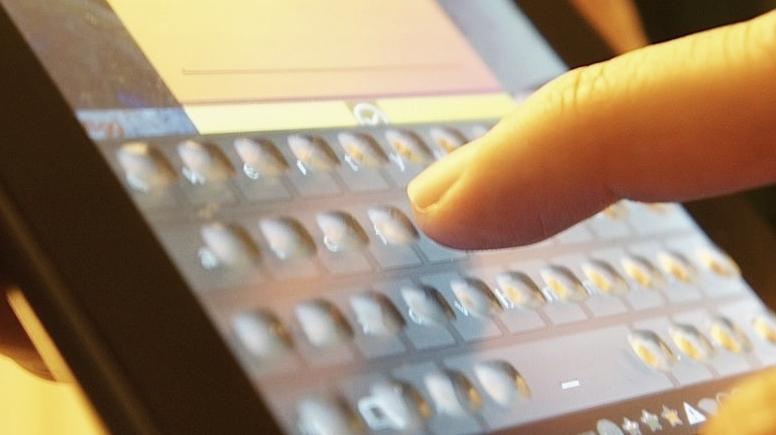
\includegraphics[width=2in]{tactus-keyboard.jpg} 
\caption{A Tactus keyboard}
\label{figure-sample}
\end{figure}

Another limitation of touchscreen devices that is frequently examined in the literature is how the human finger as a pointing device has ``very low resolution."\cite{Albinsson} With mobile touch screens in particular, research has illustrated the difficulty in pointing at targets that are often smaller than the width of the user's finger. A notable approach to tackling this problem was made by Schneiderman, Sears, and colleagues.\cite{Sears} Their basic technique provides a cursor above the user's finger tip with a fixed offset when touching the screen. The user drags the cursor to a desired target and then lifts the finger to select the targeted object. Although this technique generally allowed users to perform precise movements with less errors, the user's efficiency tended to suffer.\cite{Sears}

Many studies have purposed using a stylus (pen) to interact with touch screens instead of using a bare finger. A stylus has better ``resolution" than a finger tip and recent studies have demonstrated that pen input is emerging as a promising interaction modality for touch screens.\cite{Bi} A study by Forlines and Balakrishnan, which evaluated multiple forms of stylus input, discussed that a major drawback of this approach is the occlusion of other elements on the screen by the pen.\cite{Forlines}

Zooming is also found in the literature as a proposed solution to increase precision of touchscreen interaction. It is possible to use zooming to enlarge the information space enough so that the user can comfortably point at the target with a bare finger. A common implementation of this zooming technique is called \textit{bounding box zoom}.\cite{Albinsson} With this approach, the user first activates a zooming mode, and then draws a `bounding box' that encloses the area to be zoomed in. When the user releases the box, the system zooms and pans to the selected area and the mode switches back to pointing. 

\begin{figure}[ht]
\centering
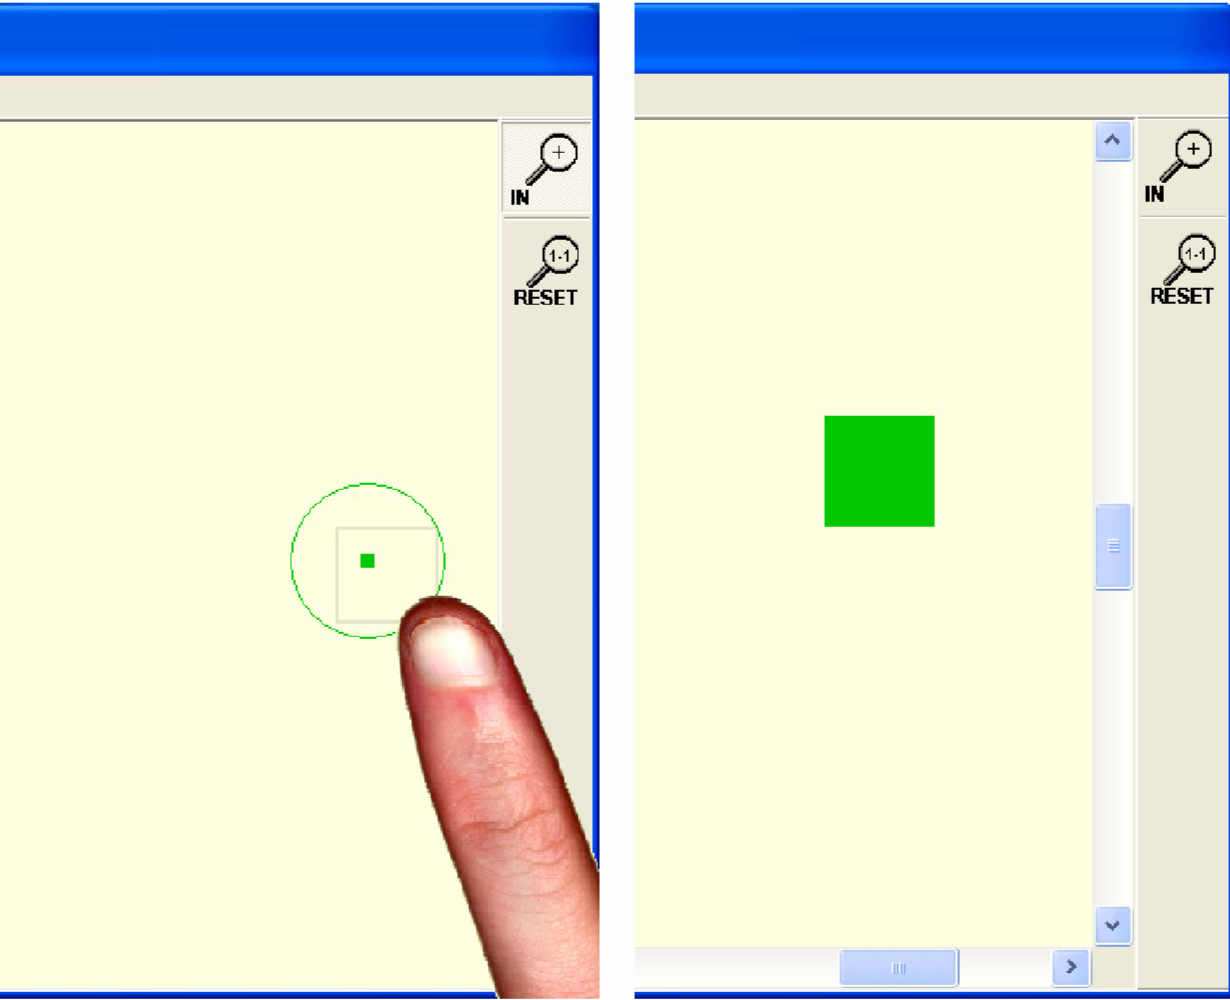
\includegraphics[width=3in]{zoom.png} 
\caption{An example of \textit{bounding box zoom}. First, the user defines the zoom area by drawing a rectangle (left). Then, the user can the perform direct pointing at a finer scale (right).}
\label{figure-sample}
\end{figure}

An example of a graphical interface that implements the \textit{bounding box zoom} technique is \textit{Pad++}.\cite{Bederson} Though the results of a study by Benjamin Bederson and James Hollan suggested that \textit{Pad++} improved users' overall touchscreen interaction precision, the device's emphasis on expandability and efficiency had certain ``learnability consequences."\cite{Bederson} 

\clearpage

\subsection{Advantages}
Previous work on the subject of touchscreen display devices not only discusses limitations and proposed solutions, but also examines advantages of touchscreen displays. Ben Schneiderman's essay, \textit{Touch Screens Now Offer Compelling Uses},  argues that touchscreen devices can be advantageous for multiple reasons: they are forms of direct manipulation, they are easy to learn, they are the fastest pointing device, no extra workspace is required to use them, etc. \cite{73754} Many experiments have been conducted that provide evidence supporting Schneiderman's reasoning. For example, the results from an experiment by Robert Hardy and Enrico Rukzio suggest that finger interaction is, in fact, faster than alternative pointing devices in most situations.\cite{Hardy:2008:TIT:1409240.1409267} A separate experiment that implemented a touchscreen electronic medical record system supported Schneiderman's assertion that touchscreen display devices are generally more learnable.\cite{Douglas:2011:SUL:2029976.2029990}


\section{Methods}

Though literature on the subject of touchscreen display devices have presented many limitations, the most relevant and important seems to be the lack of tactile features and the requirement for heightened visual attention. For people who are blind, accessing touch screen interfaces is nearly impossible. Some accessibility features are beginning to be developed though

The principle of feedback
feedback ---sending back to the user information about what action has actually been done, what result has been accomplished--- is a well-known concept in the science of control and information theory\cite{Norman02} "In the good old days of the telephone", "telephones were designed with much more care and concern for the user. Designers at the Bell Telephone Laboratories worried a lot about feedback. The push buttons were designed to give an appropriate feel---tactile feedback. When a button was pushed, a tone was fed back into the earpiece so the user could tell that the button had been properly pushed. When the phone call was being connected, clicks, tones, and other noises gave the user feedback about the progress of the call." ``All this changed." ``Why are modern telephone systems so difficult to use? Basically, the problem is that the systems have more features and less feedback"

\subsection{What Work is Most Relevant/Important?}

\LaTeX\ has support for up to three outline levels (\verb!\section!, \verb!\subsection!, and \verb!\subsubsection!).  It also recognizes \verb!\paragraph! and \verb!\subparagraph! directives, though those don't show up in the table of contents.  All of these directives expect a title.

Note also the use of the \verb!\verb! directive for inserting code-like labels or symbols.  It was particularly needed here so that we can include the backslash character in the text.

\section{Discussion}

We're adding another section just so you can see how that looks.  Plus there are a few more \LaTeX\ features to illustrate.

\LaTeX\ is very good at providing clean lists.  Examples are shown below.

\begin{itemize}
\item Bulleted items come out properly indented and spaced, every time.

\begin{itemize}
\item Sub-bullets are a virtual no-brainer: just nest another \verb!itemize! block.
\item Note how the bullet character automatically changes too.
\end{itemize}

\item Just keep on adding \verb!\item!s\ldots

\item \ldots until you're done.
\end{itemize}

Numbered lists are almost identical, except that you specify \verb!enumerate! instead of \verb!itemize!.  List items are specified in exactly the same way (thus making it easy to change list types).

\begin{enumerate}
\item A list item
\item Another list item
\item A list item with multiple nested lists

\begin{itemize}
\item Nested lists can be of mixed types.
\item That's a lot of power and flexibility for the price of learning a handful of directives.

\begin{enumerate}
\item Like nested bullet lists, nested numbered lists also ``intelligently'' change their numbering schemes.
\item Meanwhile, all \emph{you} have to write is \verb!\item!.  \LaTeX\ does the rest.
\end{enumerate}
\end{itemize}

\item Back to your regularly scheduled list item

\end{enumerate}


We may as well include a second figure also, shown in Figure~\ref{figure-sample2}.  The same image file is used, but note how it can be resized.  Again, observe how the positions of the tables and figures do not necessarily match their positions in the source file, reiterating the aforementioned \LaTeX\ functionality for deciding where these items go in the final document.  You provide an approximate location, and \LaTeX\ does the rest.


\section{Conclusions}


Wrap up your paper with an ``executive summary'' of the paper itself, reiterating its subject and its major points.  If you want examples, just look at the conclusions from the literature.
\clearpage


\bibliography{mybib}{}
\bibliographystyle{plain}
\end{document}
%%%%%%%%%%%%% end %%%%%%%%%%%%%%%%%%%%%%%%%%%%%%%


\end{document}
